%\documentstyle[epsf,twocolumn]{jarticle}       %LaTeX2.09仕様
%\documentclass[twocolumn]{jarticle}     %pLaTeX2e仕様
\documentclass{jarticle}     %pLaTeX2e仕様

%一枚組だったら[twocolumn]関係のとこ消す

\setlength{\topmargin}{-45pt}
%\setlength{\oddsidemargin}{0cm} 
\setlength{\oddsidemargin}{-7.5mm}
%\setlength{\evensidemargin}{0cm} 
\setlength{\textheight}{24.1cm}
%setlength{\textheight}{25cm} 
\setlength{\textwidth}{17.4cm}
%\setlength{\textwidth}{172mm} 
\setlength{\columnsep}{11mm}

\kanjiskip=.07zw plus.5pt minus.5pt

\usepackage{graphicx}
\usepackage[dvipdfmx]{color}
\usepackage{subcaption}
\usepackage{enumerate}
\usepackage{comment}
\usepackage{url}
\usepackage{multirow}
\usepackage{diagbox}
\usepackage{amsmath,amssymb}
\usepackage{mathtools}
\usepackage{wrapfig}


\begin{document}
  \noindent
  \onecolumn
  \hspace{1em}

  \today
  ゼミ資料
  \hfill
  \ \ B3 西村昭賢 

  \vspace{2mm}
  \hrule
  \begin{center}
  {\Large \bf 進捗報告}
  \end{center}
  \hrule
  \vspace{3mm}


\section{今週やったこと}

\begin{quote}
  \begin{itemize}
   \item 基礎実験の改良
   \item カードゲーム自体の改良の検討
  \end{itemize}
 \end{quote}

\section{基礎実験の改良}
先週の簡単な条件下の基礎実験において,思ったような学習結果を得られなかったので改良を加えて再実験した.

\subsection{ゲームのルール変更}
先週の実験が思うような結果にならなかった原因の 1 つとして考えられるのが,先攻と後攻の有利不利が激しいということである. そのため森先生に頂いたアドバイスを踏まえシャドウバースのように,相手のカードを攻撃すると攻撃したカードが反撃を食らうようにルールを変更した.

\subsection{実験条件の変更}
先攻の有利不利が激しいという問題は,カードの攻撃の仕様だけでなく事前に決定した盤面からも生まれていた.より後攻が有利になるように図\ref{fig:Figure1}のように盤面を変更した.


\begin{figure}[htbp]
  \centering
  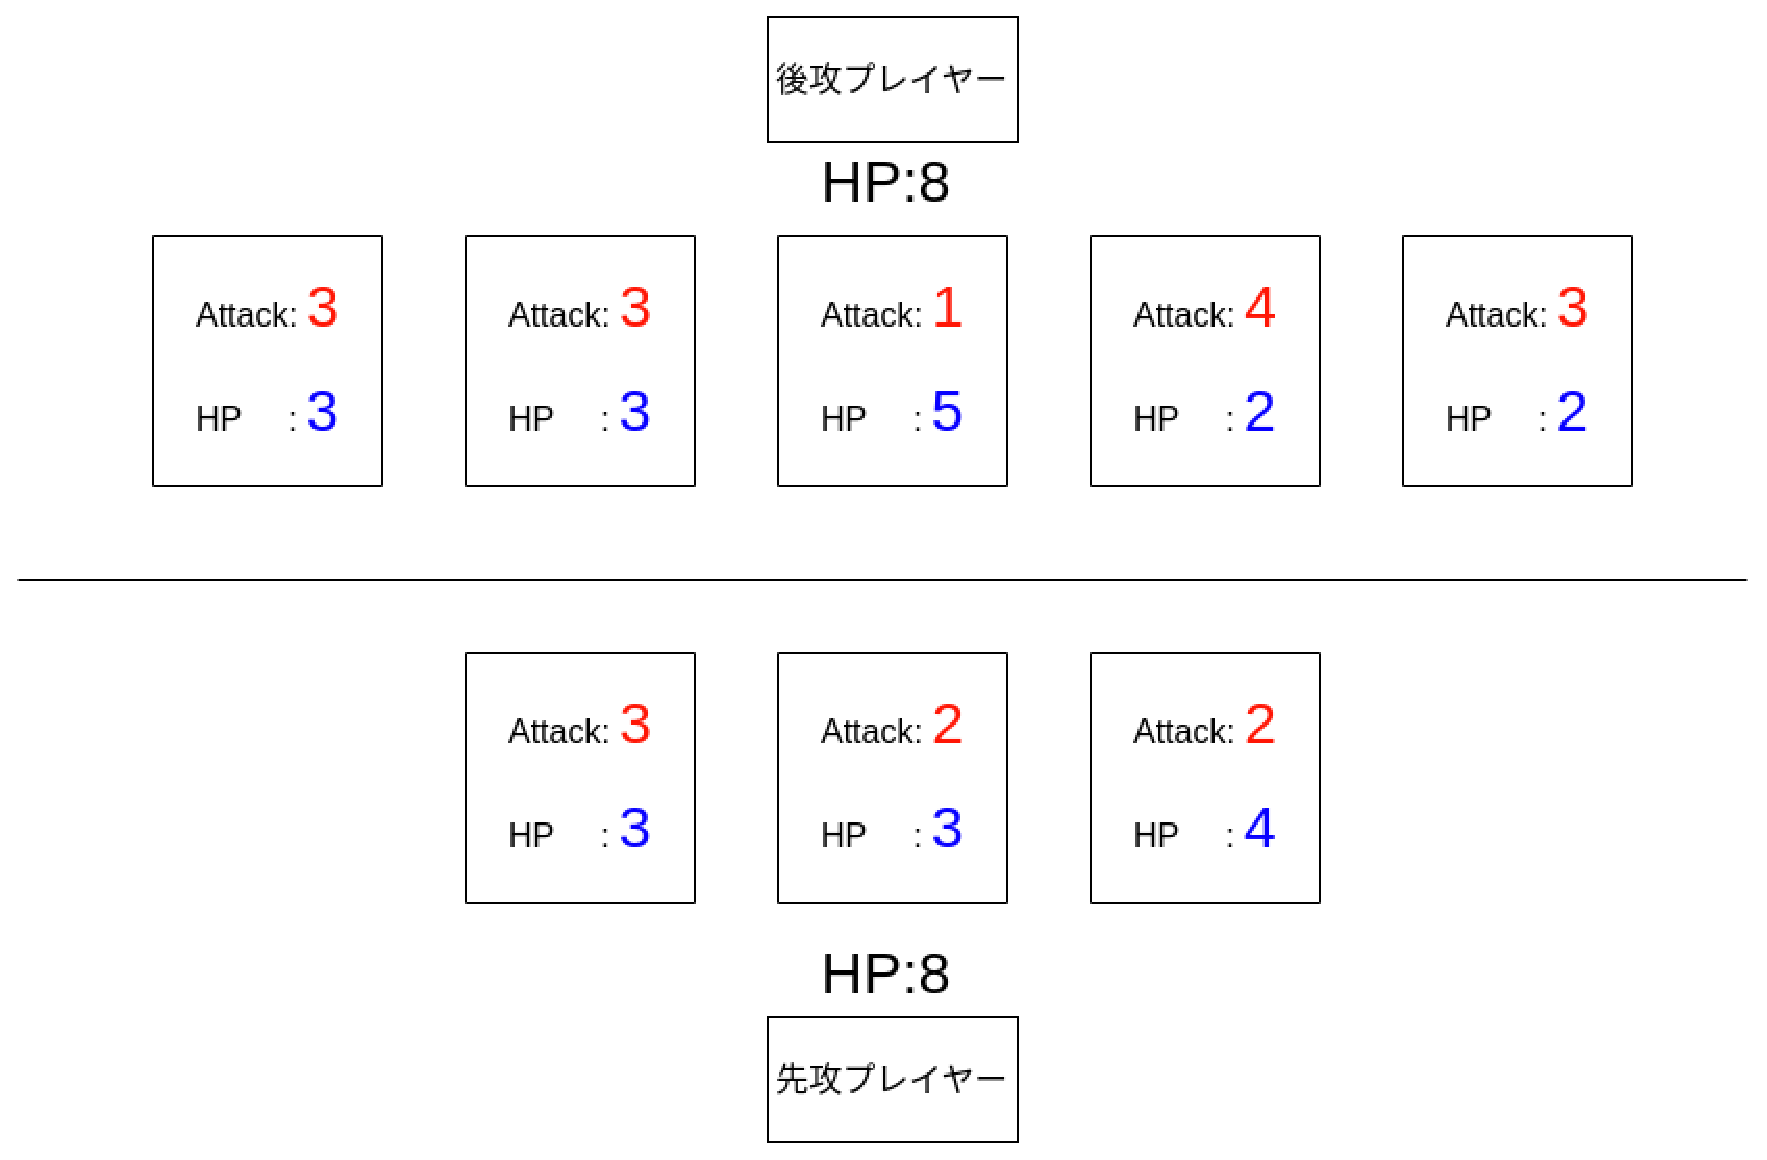
\includegraphics[width=120mm]{assets/Figure1.eps}
  \caption{基礎実験における盤面のイメージ図}
  \label{fig:Figure1}
\end{figure}

また,後攻のプレイヤーの行動は先攻プレイヤーを直接攻撃する,敵カードのどれかをランダムに選んで攻撃するの 2 種類をランダムに選ぶように変更した.

\subsection{報酬設定の見直し}
前回は盤面の評価関数と報酬設定を
\begin{equation*}
  \begin{split}
    f(\mathrm{盤面}) = 
    &\alpha*\mathrm{(自カードの評価値の和)}+\beta*\mathrm{(ターン中に削った敵プレイヤーの体力)}\\
   & - \gamma*\mathrm{(敵カードの評価値の和)} - \delta*\mathrm{(ターン中に削られた自プレイヤーの体力)}\\
    &where \qquad \alpha , \beta , \gamma , \delta \in \mathbb{R}^+
  \end{split}
\end{equation*}
\begin{equation*}
  \mathrm{エピソード終了後}
  \quad reward \text{ = }
  \left\{
    \begin{aligned}
        1 \quad &(f(\mathrm{盤面}) \geqq 0) \\
        -1 \quad &(f(\mathrm{盤面}) < 0)
    \end{aligned}
    \right.
\end{equation*}
と定めてステップ中は$reward = 0$ とし,同じ行動が続いた時は不適切として $reward = -1.0$ と設定した.

式から分かるように先週は学習を安定させるため報酬を-1.0と1.0に Cliping していた.しかしこのような報酬の Cliping を行うことで報酬の大小の大きさをエージェントが認識できない問題が生じる.そのため今週は報酬の Cliping を行わず,さらに盤面の評価関数を以下のように変更した.

\begin{equation*}
  \begin{split}
    f(\mathrm{盤面}) = 
    &\alpha*\mathrm{(自カードの評価値の和)}+\beta*\mathrm{(自プレイヤーの残り体力)}\\
   & - \gamma*\mathrm{(敵カードの評価値の和)} - \delta*\mathrm{(敵プレイヤーの残り体力)}\\
    &where \qquad \alpha , \beta , \gamma , \delta \in \mathbb{R}^+
  \end{split}
\end{equation*}
\begin{equation*}
  \mathrm{エピソード終了後}
  \quad reward \text{ = }
  \left\{
    \begin{aligned}
        -50 \quad &(自プレイヤーの体力が0以下) \\
        50 \quad &(敵プレイヤーの体力が0以下) \\
        -30 \quad &(自プレイヤーの盤面のカードの総攻撃力が敵の残り体力以上の時)\\
        f(盤面) \quad &(その他の時)
    \end{aligned}
    \right.
\end{equation*}
ステップ中は自プレイヤーの盤面のカードの総攻撃力が敵の残り体力以上の時に$reward = -50$ , ターン中に一度使おうとしたカードを使おうとした時 $reward = -3$ , 何もない時は $reward = 0$ とした.
なお,今回の実験では$\alpha = 1.0$ , $\beta = 3.0$ , $\gamma = 1.5$ , $\delta = 0.5$ とした.
\subsection{結果}
\subsubsection{実験1}
先週と同様に10000ステップ学習を行った.
図 \ref{fig:8vs8result} に実験において学習過程における 1 エピソードごとのステップ数,報酬を記録したグラフを示す.

\begin{figure}[htbp]
  \centering
  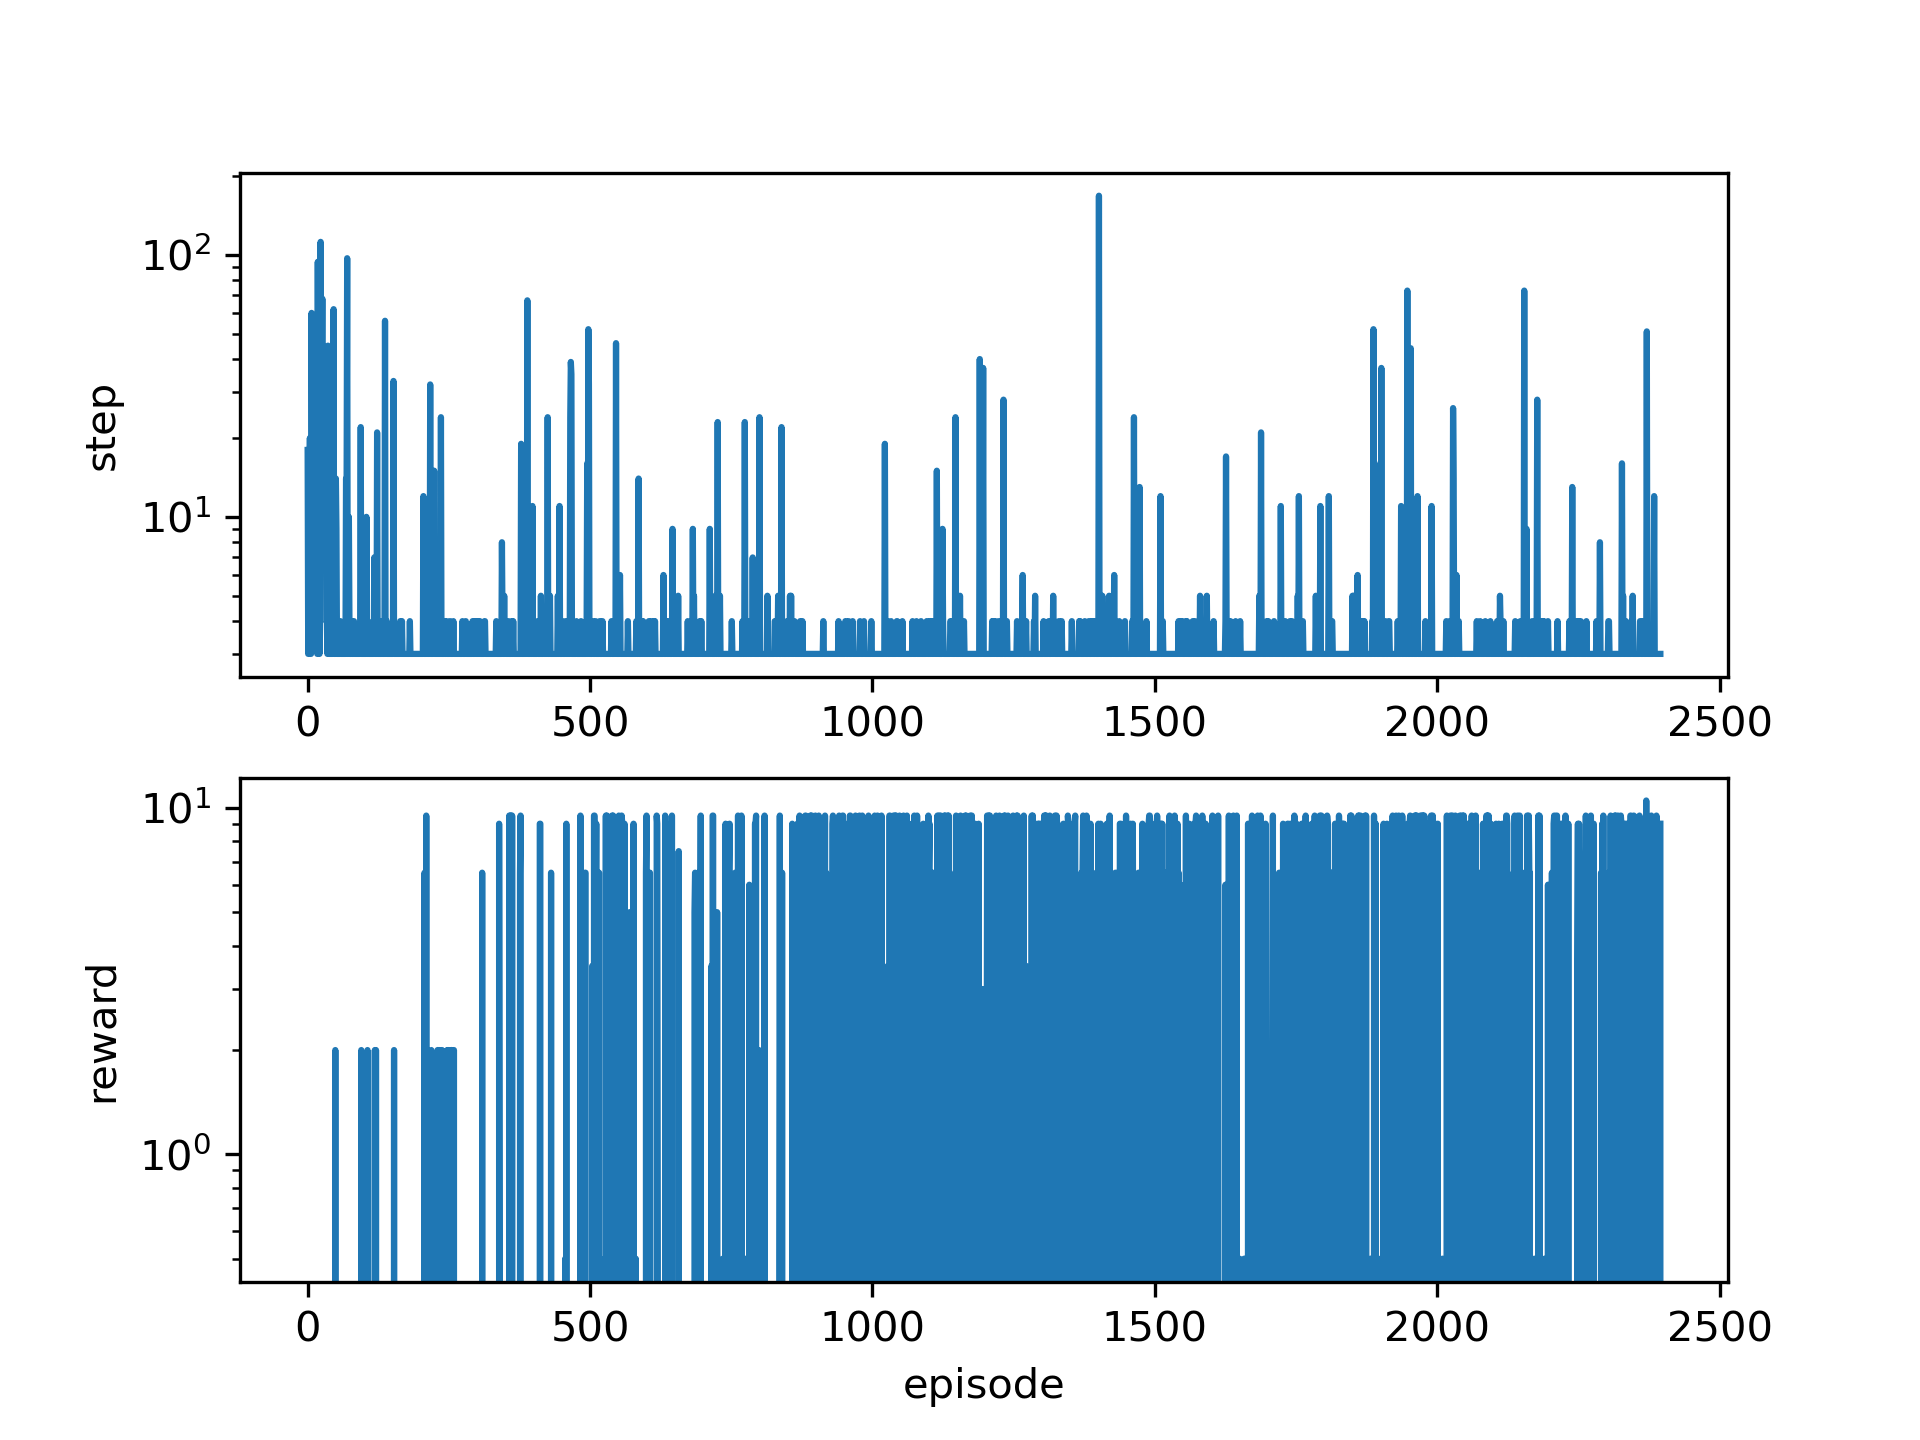
\includegraphics[width=130mm]{assets/8vs8result.eps}
  \caption{ 1 エピソードごとのステップ数,報酬 (実験 1 )}
  \label{fig:8vs8result}
\end{figure}

学習後に10回検証を行い動作を確かめた.その結果,先手のプレイヤーは
\begin{enumerate}
  \item カード (Attack , HP) = ( 2 , 3 ) で敵カード ( 4 , 2 ) を攻撃
  \item カード ( 3 , 3 ) で 敵カード ( 1 , 5 ) を攻撃
  \item カード ( 2 , 4 ) で 敵カード ( 3 , 2 ) を攻撃
\end{enumerate}
といった手順を踏んでいた.
敵プレイヤーに 1 ターンでゲーム終了されないように, かつ自盤面になるべくカードを残すように学習していることが分かる.
カード( 3 , 3 ) で敵の( 3 , 3 )カードを攻撃することも考えられるが, 敵の行動がランダムであることを踏まえてなるべく多く的となる自盤面カードを残すように動いていると考えられる.
\subsubsection{実験2}
追加で後攻プレイヤーの体力を 7 とした, すなわち先攻プレイヤーはワンターンキルが可能な条件下の実験も行った.
同様に10000ステップ実験を行い, 図 \ref{fig:8vs7result} に 1 エピソードごとのステップ数,報酬を記録したグラフを示す.
結果として,図 \ref{fig:8vs7result} の reward で 50 を記録しているように,敵プレイヤーの HP を 0 にするように学習できていた.検証の動作確認でも
\begin{enumerate}
  \item カード ( 2 , 4 ) で 敵プレイヤーを直接攻撃
  \item カード ( 3 , 3 ) で 敵プレイヤーを直接攻撃
  \item カード ( 2 , 3 ) で 敵プレイヤーを直接攻撃
\end{enumerate}
と行動していた.

\begin{figure}[htbp]
  \centering
  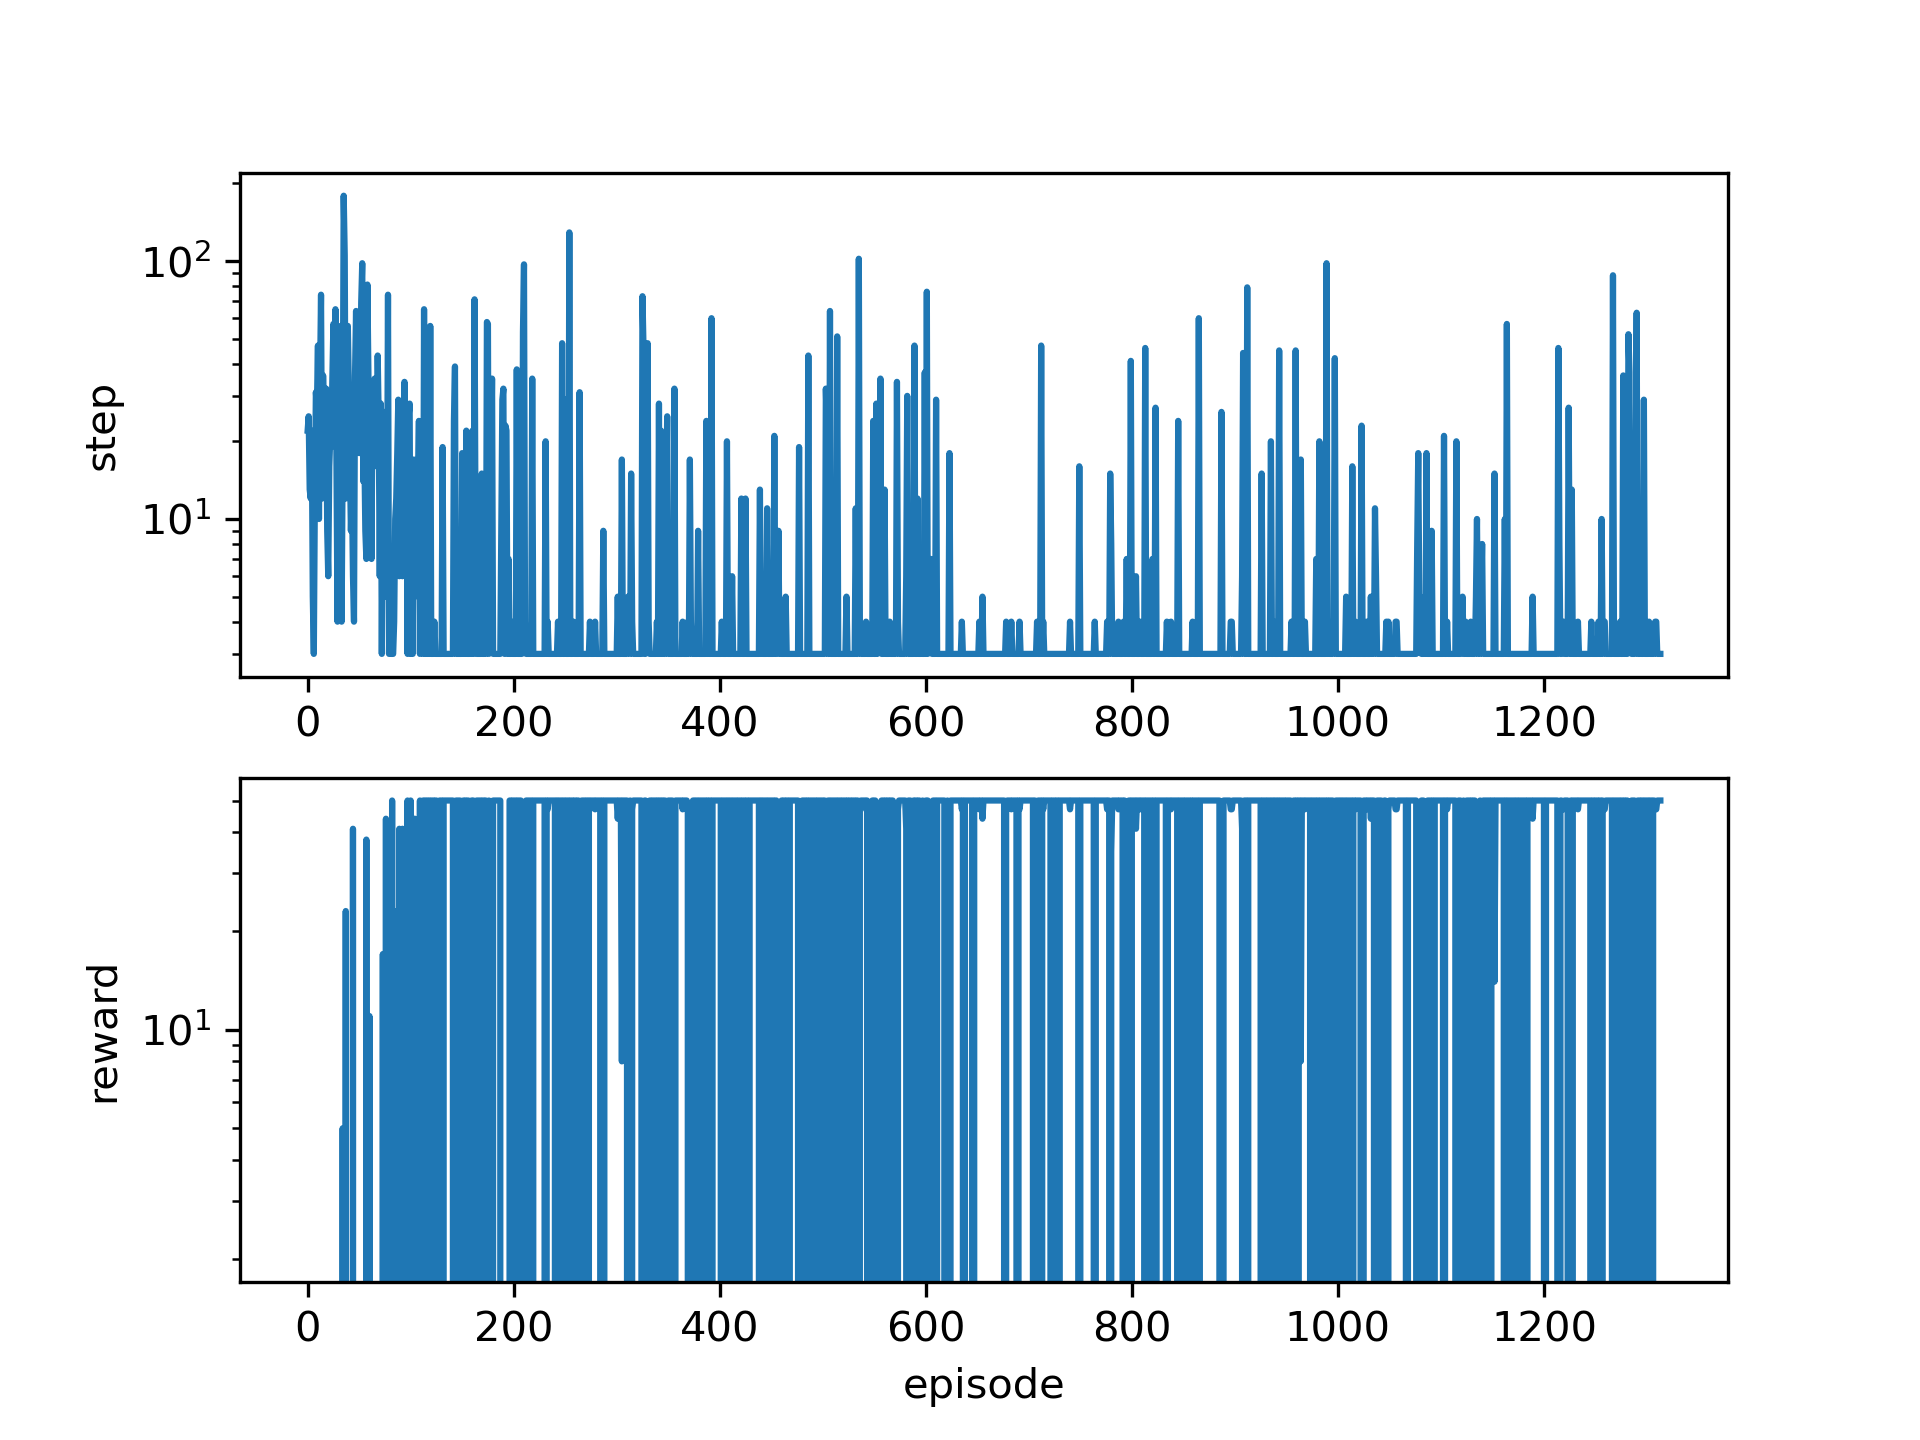
\includegraphics[width=130mm]{assets/8vs7result.eps}
  \caption{ 1 エピソードごとのステップ数,報酬 (実験 2 )}
  \label{fig:8vs7result}
\end{figure}

\section{カードゲーム自体の改良の検討}
現在は決まった盤面において先攻プレイヤーのターン,後攻プレイヤーのターンまでしか学習が行えていない.将来的にはゲーム開始からゲーム終了までを学習できるようにする必要がある.
そのためには OpenAI Gym で定義するエージェントの行動空間,状態空間を変更する必要がある.
今回は盤面を予め設計することで行動空間の次元数と状態空間のパラメータを決定する方針を考えた.

\subsection{行動空間の定義}
OpenAI Gym では行動空間の次元数,状態空間のパラメータを定義しなければならない. 毎回ターンが回ってくるたびに計算することが実装上困難であったため予め盤面を設計しその中で取りうる全ての行動数を行動空間の次元とする方法を検討した.図 \ref{fig:idea} に現在検討している盤面のイメージを示す.このように予め盤面と手札の枚数上限を決めておくことでプレイヤーの行動数を求めることができる.

\begin{figure}[htbp]
  \centering
  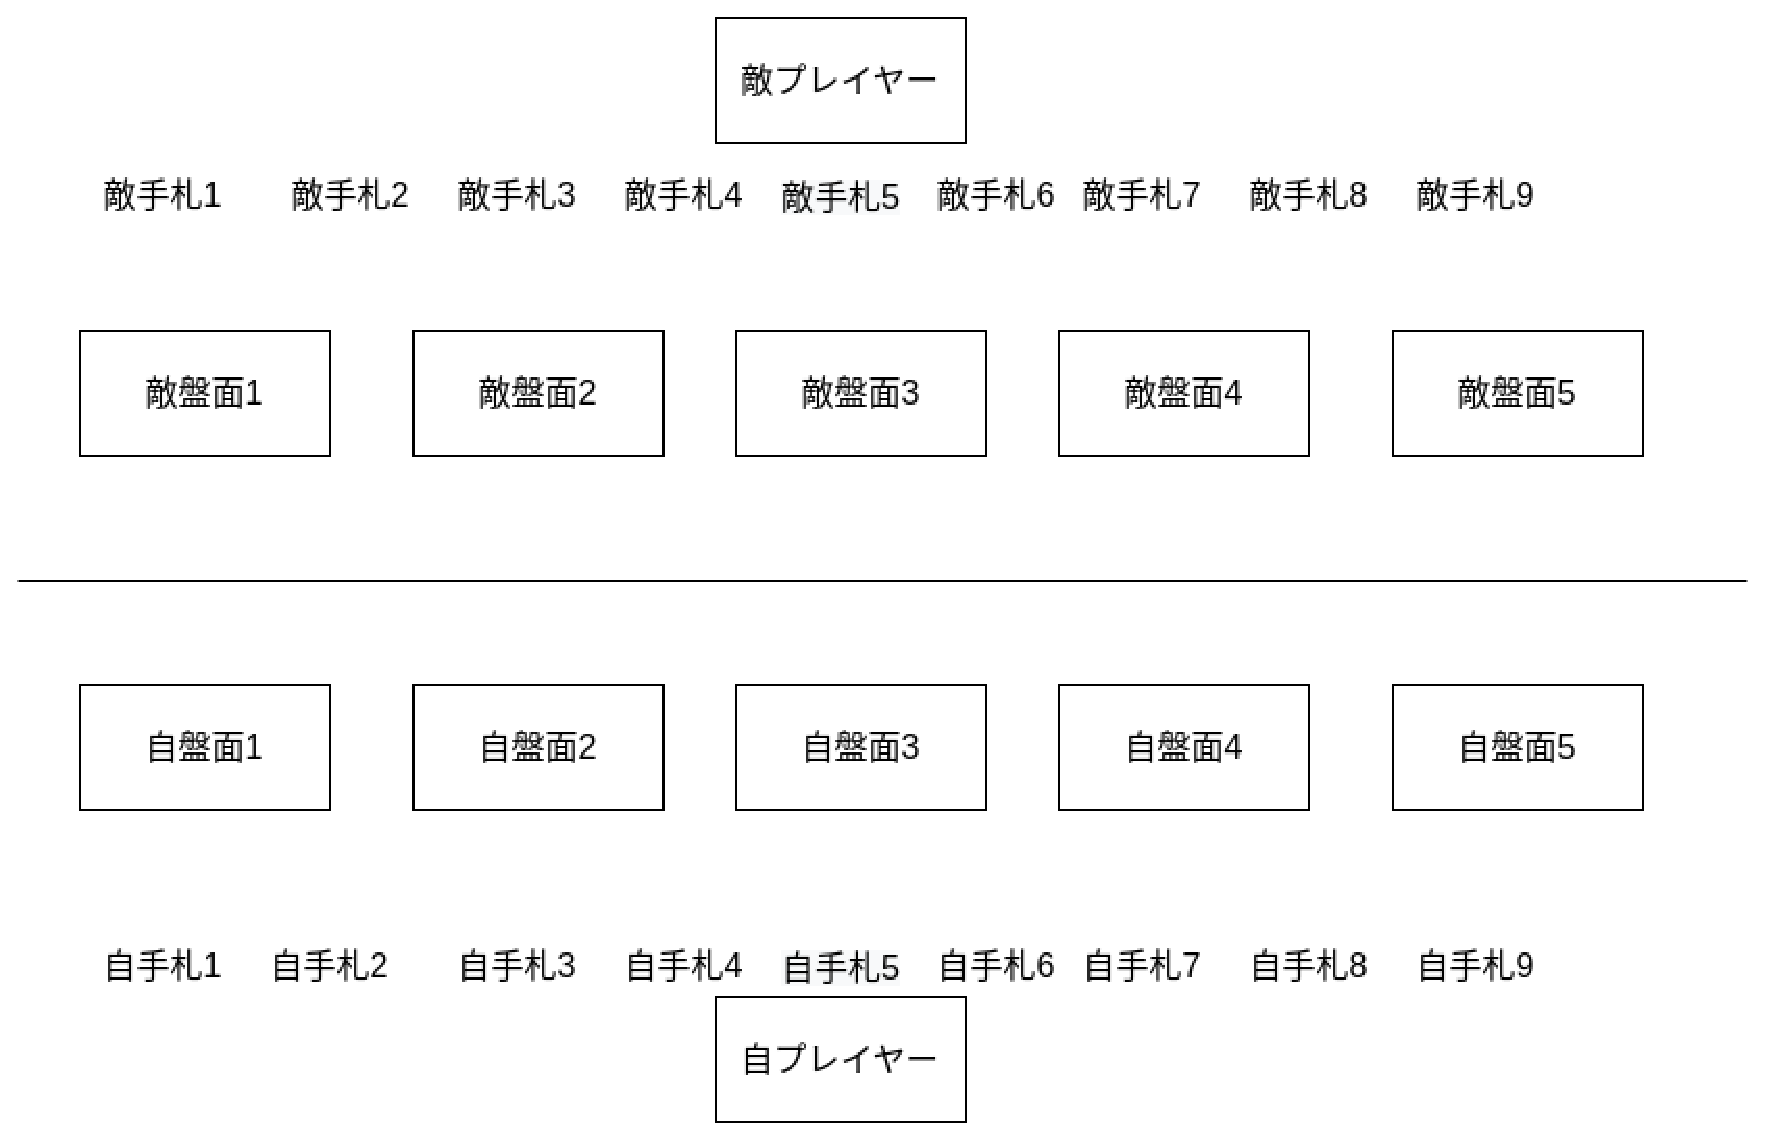
\includegraphics[width=150mm]{assets/idea.eps}
  \caption{ 検討している盤面}
  \label{fig:idea}
\end{figure}
実際に行動数を計算すると,
\begin{quote}
  \begin{itemize}
   \item 自手札のカードを自盤面に出す・・・  9*5 = 45通り
   \item 自盤面のカードが敵盤面のカードを攻撃する・・・ 5*5 = 25 通り
   \item 自盤面のカードが敵プレイヤーを攻撃する・・・ 5 = 25 通り
   \item ターンエンド・・・1通り
  \end{itemize}
 \end{quote}
の96通り考えられる.

\subsection{状態空間}
図 \ref{fig:idea} からプレイヤーが観測できる状態のパラメータとして
\begin{quote}
  \begin{itemize}
   \item 両プレイヤーの HP ,マナコスト・・・ 4個
   \item 自手札 1 ~ 9 の コスト, 攻撃力, HP ・・・ 9*3 = 27個
   \item 自盤面 1 ~ 5 の コスト, 攻撃力, HP ・・・ 5*3 = 15個
   \item 敵盤面 1 ~ 5 の コスト, 攻撃力, HP ・・・ 5*3 = 15個
   \item 自盤面 1 ~ 5 がターン中動けるかどうか ・・・ 5個
  \end{itemize}
 \end{quote}
の計 66 個のパラメータが考えられる.

\subsection{実装の際の懸念点}
行動選択時には毎ステップ時に取りうる行動を計算しなければならない.恐らく条件分岐で行動可能な行動を96個の中から全列挙しなければならないため実装量的に重そう.

\section{今後やること}


\begin{quote}
  \begin{itemize}
   \item 検討した手法の実装
   \par
    これをやらないと発展した実験ができないため最優先で行う.
    \item モンテカルロ法で解く
    \par
    実装中ではあるが Q 値の更新の箇所がちゃんと実装できていない.上手く行けばモンテカルロ木法も試して比較したい.
    \item 自動難易度調整の方法検討
    \par
    頂いた昔の修士論文は少ししか読めていないが初期パラメータの設定で進化計算を用いていた.調べたことのないアプローチだったので興味深かった.知識不足なのでいろんな論文を読んでアプローチを探っていきたい.

  \end{itemize}
 \end{quote}



%index.bibはtexファイルと同階層に置く
%ちゃんと\citeしないと表示されない(1敗)
%\bibliography{index.bib}
%\bibliographystyle{junsrt}

\end{document}